%% ============================================================ Arabic numbering

% Start page numbering at 1
\pagenumbering{arabic}
\setcounter{page}{1}

% Page style from here onwards
	\pagestyle{fancy}
	\lhead{{\sffamily \MakeUppercase\leftmark}}
	\chead{}
	\rhead{{\sffamily \MakeUppercase\rightmark}}
	\lfoot{}
	\cfoot{{\sffamily \thepage}}
	\rfoot{}
	
\chapter{Introduction}

% Textbox
\begin{center}
	\begin{tcolorbox}[title=\boxtitle]
		\begin{itemize}[leftmargin=*,labelindent=2ex,labelsep=1.5ex,itemsep=0pt,parsep=0pt]
    		\item What is the significance of the project?
			\item What does the thesis aim to achieve?
		\end{itemize}
	\end{tcolorbox}
\end{center}

%% ========================================================= Research Motivation

\section{Research Motivation}

Hearing is a fundamental sensory ability that human beings share with many other
species of the animal kingdom. The ability to perceive sound allows us to
communicate with each other vocally, detect objects in our environment without
being physically adjacent to them or having a direct line of sight, and
appreciate the melodies and harmonies of music. These qualities have established
the sense of hearing as one of our primary means of gathering information about
the world around us.

\subsection{The Bigger Picture}

Unfortunately, many people suffer from impaired hearing capabilities. In 2012,
the World Health Organisation (WHO) estimated that 360 million people worldwide
(or 5.3\% of the world's population) were afflicted with \emph{disabling hearing
loss}, defined by the WHO as more than 40~dB loss \emph{in the better hearing
ear} in adults, or 30~dB in children (see
Table~\ref{table:hearing_loss_classification})~\cite{who2012}.

\begin{table}[p]
	\centering
	\sffamily
	\small
	
	\caption[Classification of hearing loss]{Classification of hearing loss.
	(Reproduced from World Health Organisation~\cite{mathers2000}.)}
	\label{table:hearing_loss_classification}
	
	\begin{tabular}{l c l}
		\toprule
		\textbf{Grade}	& \textbf{Loss in better ear} 	& \textbf{Description} \\
						& \textbf{(dB)} 				& \\
		\midrule
		
		Normal			& $ \leq $25 	& No or very slight hearing problems; 
											able to hear whispers \\
		Mild			& 26--40		& Able to hear and repeat words spoken 
											in normal voice at 1 metre \\
		Moderate		& 41--60		& Able to hear and repeat words using 
											raised voice at 1 metre \\
		Severe			& 61--80		& Able to hear some words when shouted 
											into better ear \\
		Profound		& $ \geq $81	& Unable to hear and understand even a 
											shouted voice \\
		\bottomrule
	\end{tabular}
\end{table}

In Australia alone, over 422,000 individuals (representing 2.1\% of the
population) were classified as being at a similar level of hearing loss (more
than 45~dB loss in adults, or 30~dB in children) in 2005~\cite{economics2006}.
By 2050, this figure is predicted to increase to just shy of 1 million people
(3.4\% of Australia's projected population), as shown in
Figure~\ref{fig:HL_prevalence}. (Note that these Australian numbers are
underestimates relative to the WHO definition due to the more stringent
criteria and earlier sample time.)

\begin{figure}[p]
	\centering
	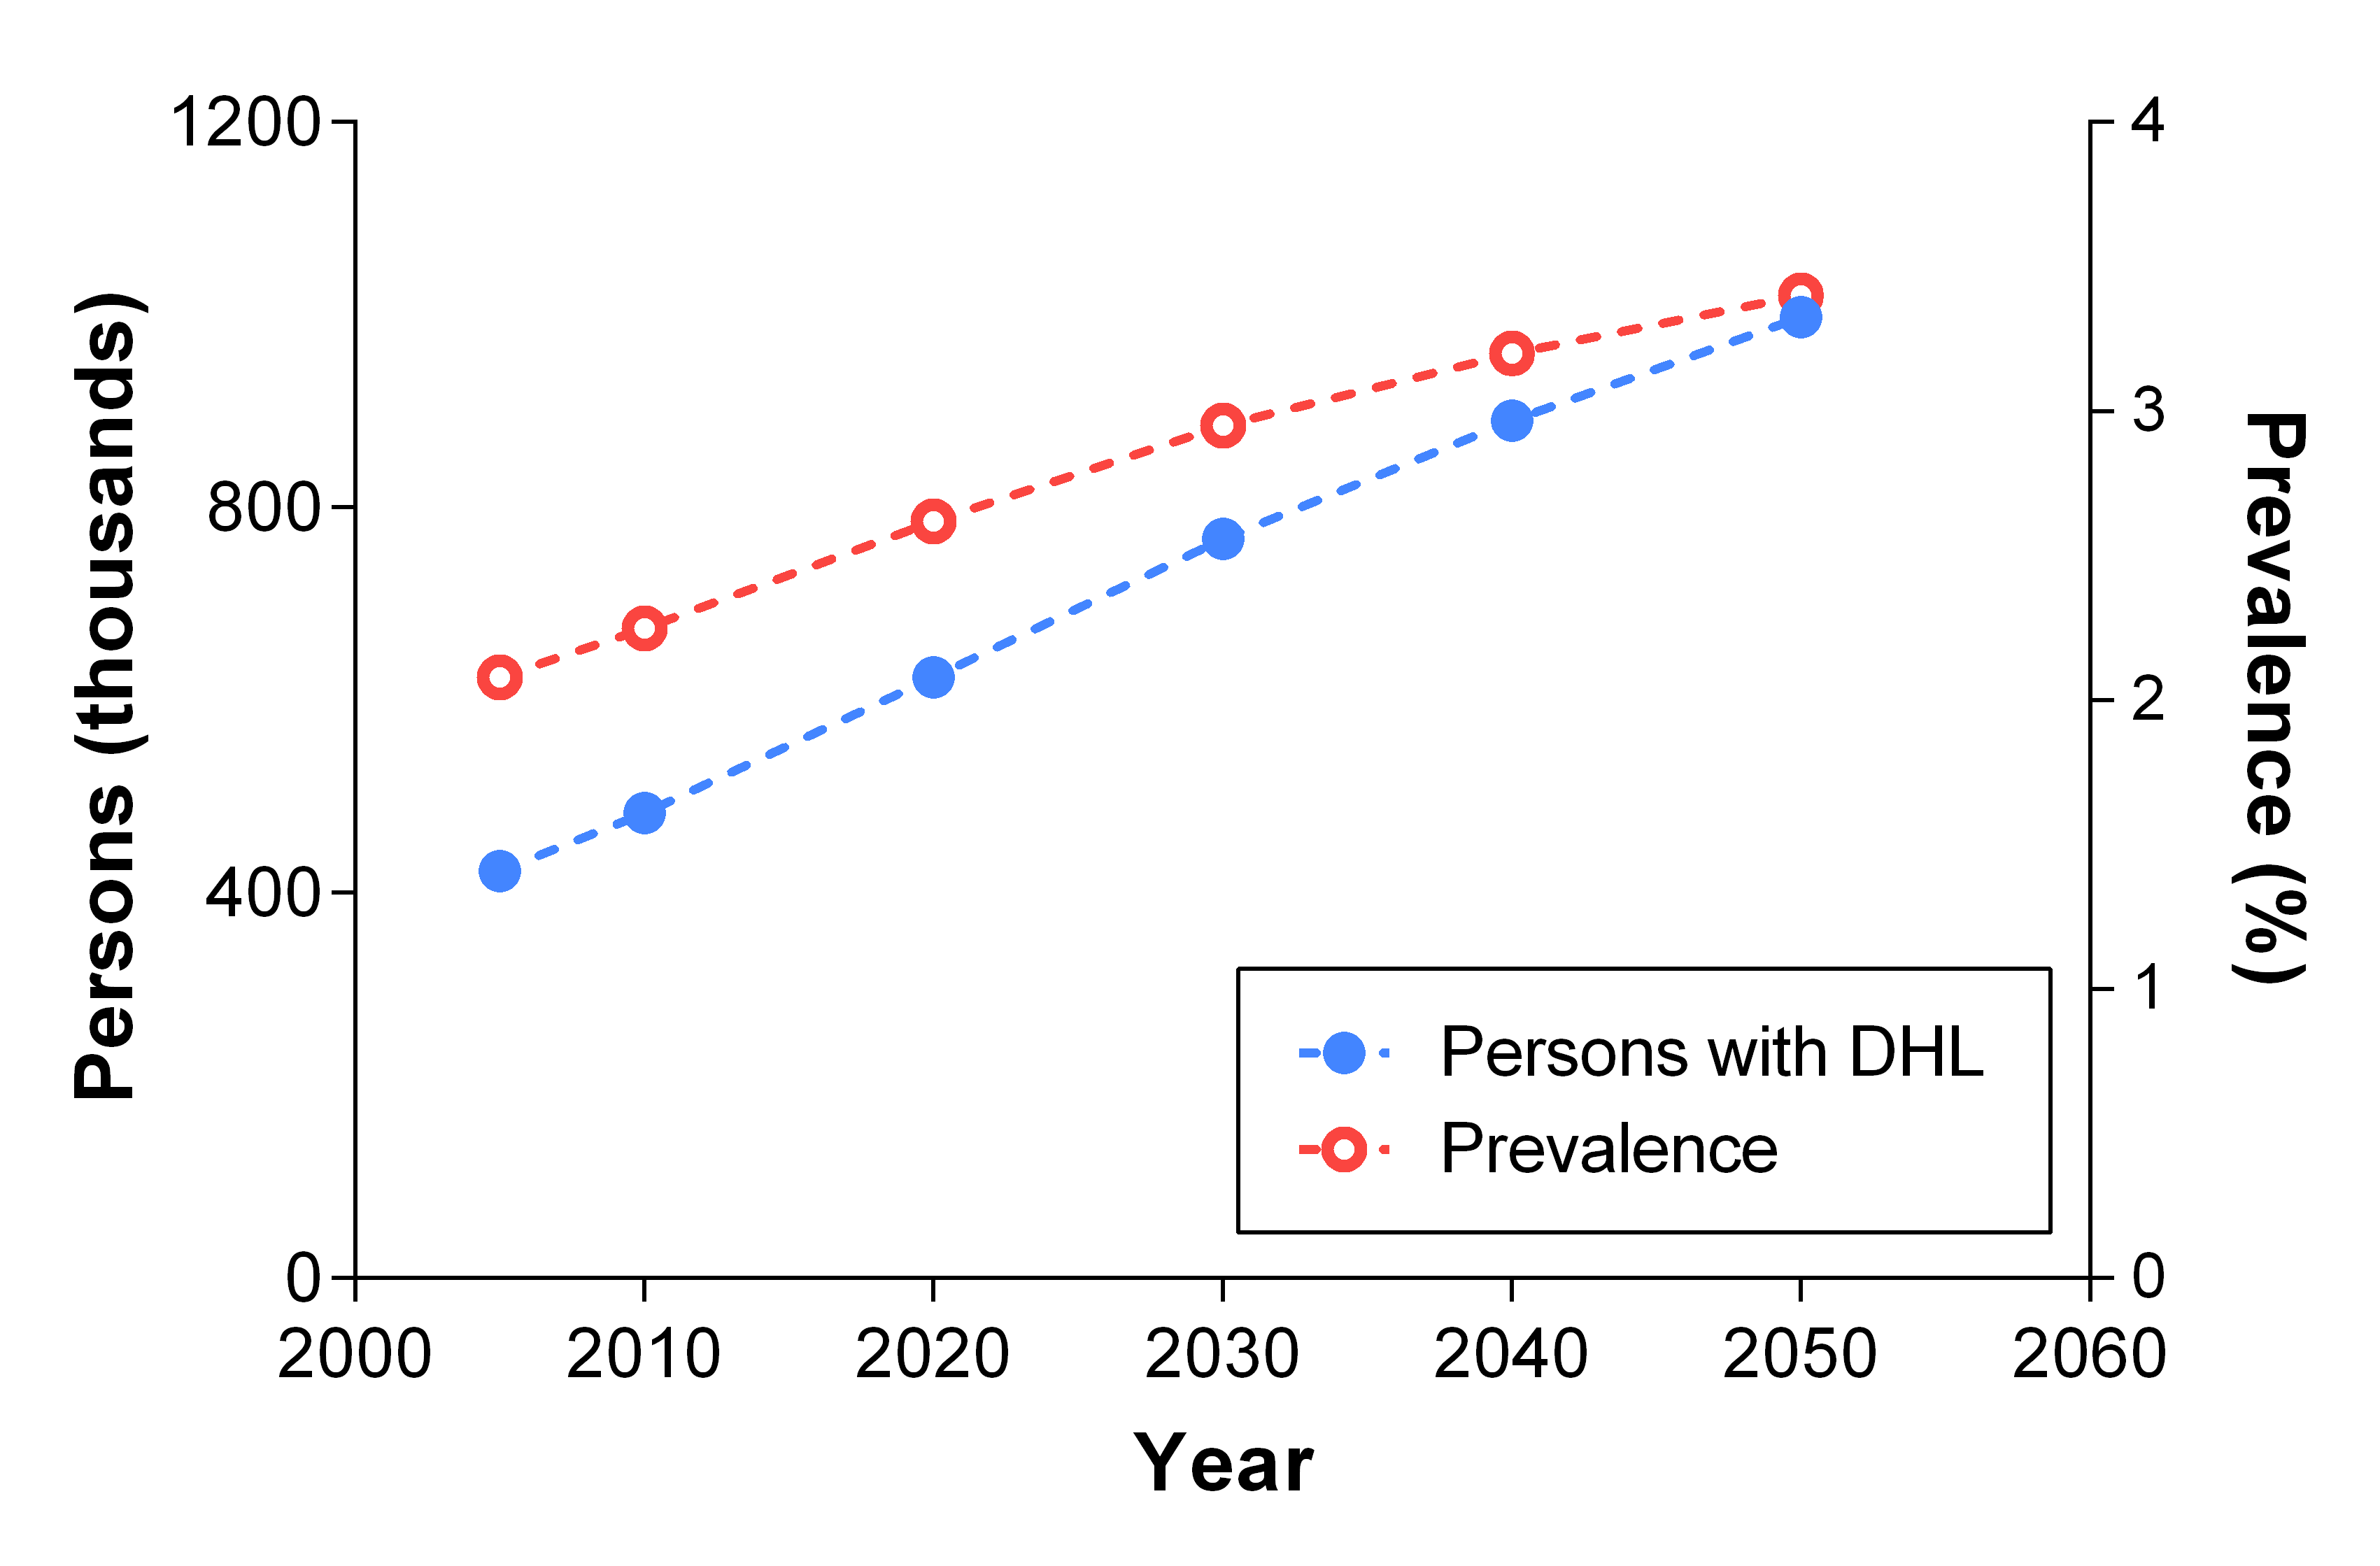
\includegraphics[height=8cm]{Introduction/hl_prevalence}
	\caption[Projected prevalence of disabling hearing loss in Australia]{Projected
	prevalence of disabling hearing loss (DHL) in Australia, 2005--2050. (Data from
	Access Economics~\cite{economics2006}.)}
	\label{fig:HL_prevalence}
\end{figure} 

Hearing loss comes with a number of personal costs to affected individuals in
addition to the reduced capacity to communicate. Quality of life is reduced
through suffering and loss of leisure~\cite{economics2006}. Participation in
education, skill development, and employment are hindered, putting pressure on
their consumable incomes which are, as a group, already lower than
average~\cite{economics2006}. Families, friends, and co-workers interacting with
the hearing impaired person are also affected, which can cause some individuals
to feel like they are a burden on those around them~\cite{mo2005}. Social
isolation is also well documented, and can lead to emotional tolls through
anxiety and depression~\cite{mo2005}.

The financial costs associated with hearing loss are
substantial~\cite{economics2006}. It was estimated to cost the Australian
economy about \$11.75 billion (1.4\% of gross domestic product) in 2005. The
largest component of this cost is productivity loss (\$6.7 billion), followed by
informal carers (\$3.2 billion), deadweight losses (\$1.0 billion), and then
direct health system costs (\$674 million). In addition to these numbers, the
monetary value corresponding to the loss of wellbeing described in the previous
paragraph was estimated to be some \$11.3 billion~\cite{economics2006}.

Considering the millions of people affected around the world, these Australian
estimates only represent a small fraction of the global total. It would appear
that the restoration of hearing capabilities would yield significant benefits
not only for affected individuals, but also for the economy as a whole. Indeed,
treatments for hearing loss are reportedly very cost-effective
interventions~\cite{economics2006}.

\subsection{The Cochlear Implant Performance Plateau}

Roughly 90\% of hearing loss is sensorineural in nature~\cite{wilson1998}, as
described in \S\ref{sect:hearing_loss}. For those categorised as having severe
or profound \emph{sensorineural hearing loss} (SHL), the cochlear implant (CI)
is the only effective treatment. Unlike hearing aids, which simply amplify
incoming sound signals, CIs work by injecting pulses of electric current into
the inner ear to stimulate auditory neurons directly
(\S\ref{sect:cochlear_implants}). The United States Food and Drug Administration
(FDA) reported that as of December 2012, approximately 324,200 people worldwide
had received CIs~\cite{nidcd2014}, and it is expected that this number will
continue to grow.

The quality of sound perception has shown marked improvements since CIs were
first developed. Figure~\ref{fig:sentence_recognition} shows the trend in
sentence recognition scores in quiet environments for CI recipients using
various sound processing strategies from the top device
manufacturers~\cite{zeng2008}. There were (and still are) significant variations
in speech performance amongst individuals~\cite{loizou1998}, but innovations in
the processing of speech signals~\cite{wilson1991nature,clark1996, loizou1998}
were able to produce rapid jumps in average performance over the first one and a
half to two decades of CI development.

\begin{figure}
	\centering
	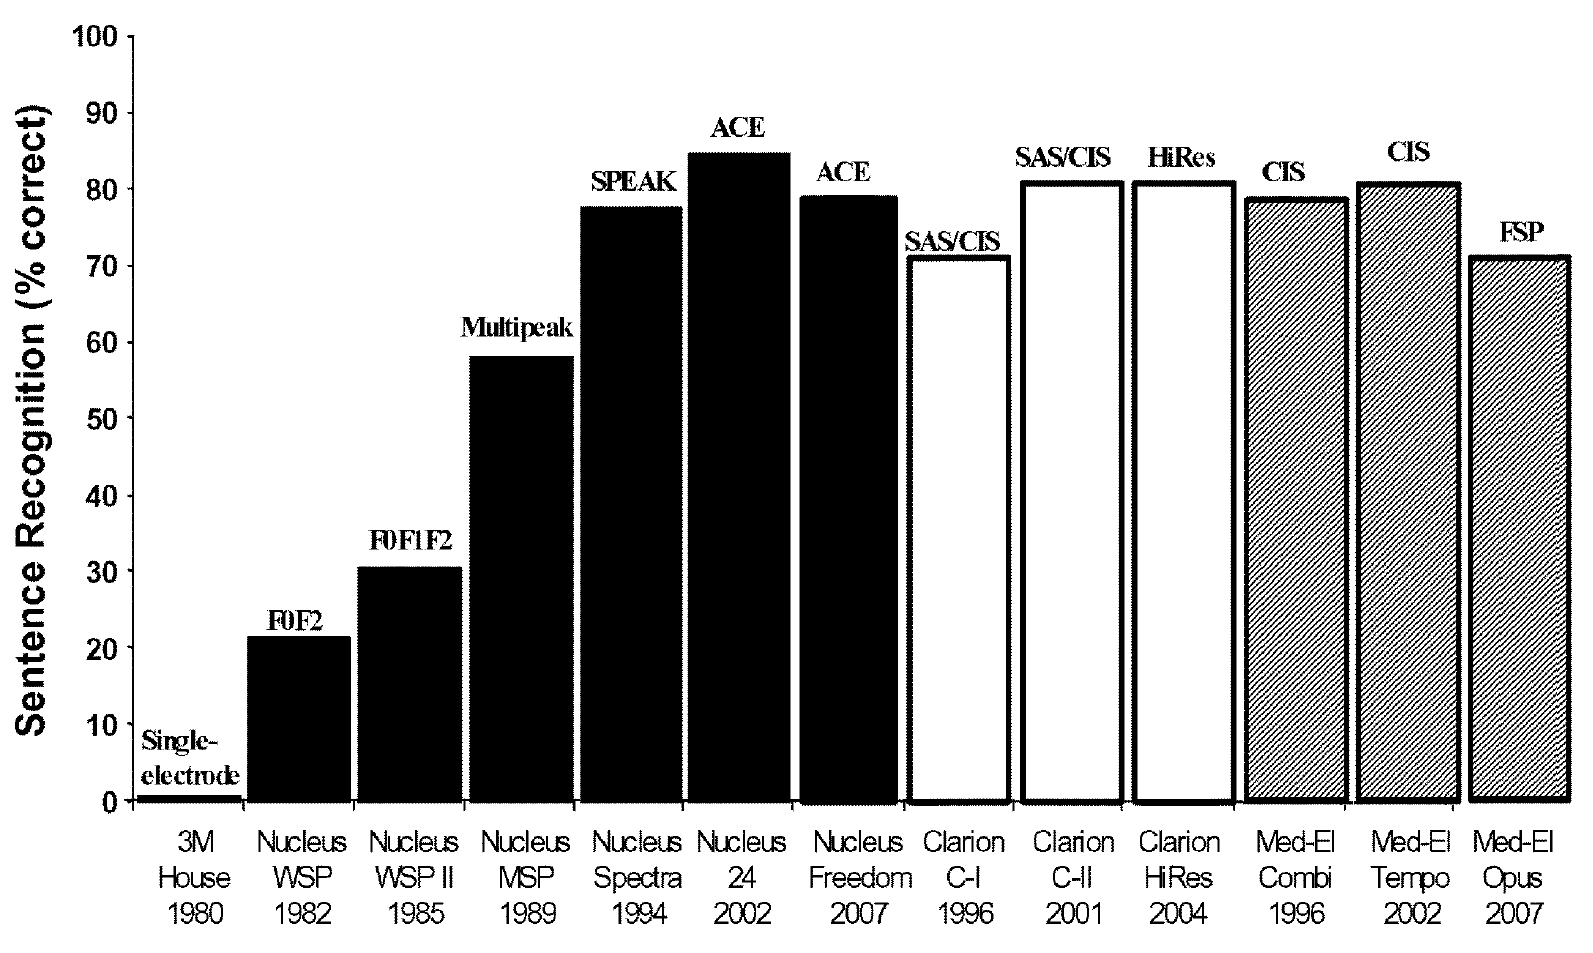
\includegraphics[height=8cm]{Introduction/sentence_recognition}
	\caption[Sentence recognition scores in quiet since 1980]{Sentence recognition
	scores in quiet since 1980. (Source: Zeng~\cite{zeng2008}. Copyright 
	\textcopyright{} 2008, IEEE.)}
	\label{fig:sentence_recognition}
\end{figure} 

Despite the technological merits of newer schemes, however, speech performance
in quiet has since plateaued~\cite{seligman2004,vandenhonert2007,zeng2008}. One
reason for this may be a shift in research focus towards improving other use
cases---with a large portion of users experiencing adequate performance in
quiet, researchers began working on performance in noisy environments, pitch
discrimination (for music and tonal languages), and other fringe cases to make
the implants more robust and relevant to the everyday lives of implant
recipients.

There may however be another potential explanation. Consider that the mechanism
ultimately responsible for hair cell stimulation is the \invivo{} current flow
(cf. \S\ref{sect:cochlear_implants}). The spatial distribution of this flow is
largely dictated by three factors: the design of the intracochlear electrode
array, its position within the cochlea after surgical insertion, and the
electrical properties of the tissues around the implant. The design of the array
is arguably the most important of these because it can affect both the
intrascalar positioning of the electrode array and, at least in part, the
surrounding tissue
response~\cite{miller1997,tykocinski2000,briggs2001,vanderbeek2005,
wardrop2005a,wardrop2005b,richardson2009}.

CI array designs have remained relatively stagnant in comparison to speech
processing techniques~\cite{girzon1987, micco2006, whiten2007}. This is not to
say that there has been zero progress in the area, but rather that the results
of such endeavours have failed to produce comparable successes. Part of the
reason for this may be a lack of impetus because early multichannel arrays were
more than sufficient to deliver the then-crude speech signals from the implant
electronics. Case in point, sentence recognition scores of over 90\% could be
obtained in quiet with just four active channels~\cite{shannon1995, dorman1997}.
As such, implants were designed with a 70 year life span [Cochlear Limited,
internal communication] in anticipation that software upgrades could be relied
on to improve performance.

With the sophistication of the latest algorithms corresponding to rather static
speech performance metrics, it would seem that the bottleneck has shifted to
other components of the system~\cite{clark2008,clark2013}. Whether these
limitations are due to array design or biological factors is not clear since the
influence of individual factors is difficult to ascertain~\cite{loizou1998}, but
it is most likely a combination of these. In either case, existing intracochlear
array designs have reached a limit, and a lack of insight into how they might
be further improved has hindered their continued development.

%% ================================================================== Objectives

\section{Thesis Goals}
\label{sect:thesis_goals}

\subsection{Enabling Knowledge Development via Computational Modelling}
\label{sect:knowledge_dev}

Traditional \invivo{} and \invitro{} methods for investigating biological
phenomena are difficult to implement in the cochlea because it is small,
contains a number of delicate structures, and is surgically inaccessible, being
encased in the densest and hardest bone in the body~\cite{bast1949, dallos1996}.
For the purposes of CI design, it is of interest to determine spatially
distributed field quantities~\cite{vanpoucke2004identification}. This presents
two main challenges to the experimentalist. Firstly, obtaining these
measurements using \invivo{} or \invitro{} methods can be impractical because
the probes must be physically placed at the location of the
measurements~\cite{girzon1987,kral1998}, a process which inherently compromises
the integrity of the cochlear structures. Most experiments therefore only
involve taking measurements within the fluid chambers of the cochlea, but even
then, introducing the probes requires perforation of either the otic capsule
surrounding the cochlea or the round window membrane and can damage the other
soft tissue structures lying within~\cite{black1980} or lead to cerebrospinal
fluid (CSF) contamination~\cite[p. 113]{salt1986}. Secondly, it is difficult to
precisely control the positioning of the probe to obtain the large number of
sample points needed for building a detailed electroanatomical map.

Over the past few decades, another method has become viable: computational
modelling, also referred to as \insilico{} experimentation. The progression of
``Moore's Law'', which predicts a doubling of the number of transistors in an
integrated circuit every two years~\cite{moore1998}, has led to a exponential
increase in processing power since the 1970s, enabling a range of numerical
methods (\S\ref{sect:numerical_methods}) to be adapted to engineering analysis.
Although the earliest \insilico{} studies were relatively simple abstractions,
the complexity of analyses that could be performed has increased over time,
spurred by the development of more robust software that took advantage of the
ever-increasing hardware capabilities.

A virtual representation of the implanted cochlea would be a useful tool for CI
research~\cite{girzon1987,micco2006,hanekom2015ciap} because it can provide an
alternative and complementary form of investigation that is not subject to the
shortcomings of traditional methods discussed above. Being able to manipulate a
virtual space means that measurements can be made in hard-to-reach places
(within Rosenthal's canal, for instance) without disturbing the surrounding
tissues, thereby providing a better representation of the \invivo{} situation.
In addition, more intuitive visualisations of the underlying bioelectric
phenomena can be produced, making the dissemination of new insights easier and
more accessible to a wider audience. When used in conjunction with \invivo{}
studies and bench-top testing, \insilico{} studies are invaluable for obtaining
a holistic understanding of medical
devices~\cite{kral1998,schimpf1998,fda2012,saba2012}.
To that end, the first goal of this project is \emph{to develop a realistic
computational model of the implanted cochlea}. All of the work that went into
producing the models in this thesis is documented in
Chapter~\ref{sect:modelling}.

Existing models of the implanted cochlea have a strong focus on explaining the
clinical outcomes observed in subjects, which is a significant and worthwhile
objective in itself, but in doing so they provide little insight into the
intermediate step of how injected current flows through the tissue both
spatially and temporally. This intermediate step must be understood in order to
gain insights that can be fed into the design process for next generation
intracochlear electrode arrays~\cite{girzon1987, schimpf1998}. It is hoped that
by analysing the relationships between the stimulating pulse, the anatomy of the
cochlea, and the electrophysiological response using computational techniques, a
more advanced understanding of the underlying mechanisms will be developed,
leading to improved intracochlear array designs that provide higher quality
sound perception, greater power efficiency, and other benefits to CI recipients.
To be clear, this is a longer term view for the industry. The focus for this
project is to develop the groundwork, methodology, and models that would enable
this future to take place.

\subsection{Addressing Untested Assumptions in the Literature}

Consider the following quote from statistician George Box: 

\begin{verse}

	\textit{
		``Essentially, all models are wrong, but some are useful. \hphantom{This is
		some filler text} \ldots the approximate nature of the model must always be
		borne in mind.'' }

 	\vspace{4mm}
	\raggedleft{
		--- George Box, 1987~\cite{box1987}
	}
\end{verse}

All models are, by definition, simplifications of reality. Sophisticated models
may approach the reality of nature, but they will never replicate it entirely;
nor should they, given that the purpose of modelling is to make complexity more
intuitive [Lianne Cartee, personal communication]. For practical purposes, what
matters is whether or not they are representative of the system being studied.

Simply creating a model does not provide an adequate foundation for further
investigation. As noted in \S\ref{sect:validation_intro}, there is some
entrenched reluctance to trust computational models in the CI research
community, despite the benefits and insights that they can provide. It is
suspected that this is due to the use of untested assumptions in existing models
that are often not intuitive nor properly justified. Coupled with the
inconsistent predictions of psychophysical outcomes from one model to the next,
which are inevitable given the multiple layers of abstraction and the difficulty
of representing biophysical interactions mathematically, it is understandable
that these doubts exist.

Hence, the second goal of this project is \emph{to critically evaluate some of
the assumptions currently used in volume conduction models of the cochlea}.
These include the impact of boundary conditions
(Chapters~\ref{sect:boundary_conditions} and \ref{sect:validation}), material
properties (Chapter~\ref{sect:validation}), vascular structure
(Chapter~\ref{sect:vascular_structure}), and time-dependent effects
(Chapter~\ref{sect:time_dependency}). Sensitivity studies will be performed to
gauge the certainty of cited input parameters, and \invivo{} measurements will
be acquired and compared with the \insilico{} results to provide guidance on
acceptable model outputs. By addressing these outstanding issues in a thorough
and logical manner, it is hoped that some of the concerns surrounding the use of
\insilico{} models may be alleviated. The outcome of these assessments will act
to either further validate existing models, or prompt changes in future models.
In either case, the profile and trustworthiness of computational models of the
implanted cochlea will be improved.


% On the other hand, the approach is also subject to several limitations <list
% cons --- realism, material properties of anisotropic biological tissues>.
% ~\cite{martini2006,johnson2006}

% Still problems to be overcome in bioelectric modelling: Potratz
% paper?~\cite{potratz2010}

% The complexity of human anatomy is further compounded by the variability between
% individuals \cite{lau2011}; this is true also for the cochlea, which despite
% being one of the smallest organs in the human body still exhibits significant
% disparities \cite{axelsson1968}

%% ========================================================== Document Structure

\section{Dissertation Structure}

The structure of the dissertation is as follows:

\begin{description}
	\item[\textsf{Chapter 1}] Explains the motivation behind the project and the
	goals of the thesis.
	\item[\textsf{Chapter 2}] Reviews the anatomy of the ear and the processes
	responsible for hearing.
	\item[\textsf{Chapter 3}] Introduces cochlear implants, examines existing work
	in bioelectric modelling to develop the reader's knowledge of the subject
	matter, and reviews the current state-of-the-art.
	\item[\textsf{Chapter 4}] Documents the methodology used to construct the
	models in the thesis.
	\item[\textsf{Chapter 5}] Examines the impact and accuracy of various
	boundary condition assumptions.
	\item[\textsf{Chapter 6}] Assesses the validity of the guinea pig cochlea model
	to ensure that input parameters and corresponding results are reasonable.
	\item[\textsf{Chapter 7}] Investigates the role of vascular	structures in
	volume conduction.
	\item[\textsf{Chapter 8}] Evaluates the feasibility of modelling
	time-dependent effects and the repercussions of these dynamics.
	\item[\textsf{Chapter 9}] Summarises the findings of the thesis and proposes
	directions for future research efforts.
\end{description}
